% $HeadURL$

%%%%%%%%%%%%%%%%%%%%%%%%%%%%%%%%%%%%%%%%%%%%%%%%%%%%%%%%%%%%%%%%%%%%%%
%%%%                   Complex
%%%%%%%%%%%%%%%%%%%%%%%%%%%%%%%%%%%%%%%%%%%%%%%%%%%%%%%%%%%%%%%%%%%%%%

\subsection{Glyph: \glyph{Complex}}\label{sec:complex}

A \glyph{complex} represents a pool of biochemical entities, each composed of other biochemical entities, whether macromolecules, simple chemicals, multimers, or other complexes. The resulting entity may have its own identity, properties and function in an SBGN map.
The \glyph{complex} can be described by the set of \glyph{subunits} \add{(\sect{subunit})} it contains (see \fig{complexSubunits}). This description is entirely optional and is there to assist the user with a visual shorthand about the composition of the complex.
% \rougny{Chaneg first sentence to ``A complex represents a pool if biochemical entities, each composed of other biochemical entities...''?}

\begin{glyphDescription}

\glyphSboTerm
SBO:0000253 ! non-covalent complex

\add{
\glyphIncoming
Zero or more \glyph{production} arcs (\sect{production}).
}

\add{
\glyphOutgoing
Zero or more \glyph{consumption} arcs (\sect{consumption}), \glyph{modulation arcs} (\sect{modulations}), \glyph{logic arcs} (\sect{logicArc}), or \glyph{equivalence arcs} (\sect{equivalenceArc}).
}

\glyphContainer
\corr{A \glyph{complex} possesses its own container box surrounding the juxtaposed container boxes of its components.
This container box is a rectangle with cut-corners (an octagonal box with sides of two different lengths). The size of the cut-corners are adjusted so that there is no overlap between the container and the components. The container boxes of the components must not overlap.}{
A \glyph{complex} is represented by a rectangular shape with cut-corners (that is, an octogonal shape with sides of two different lengths).
If the \glyph{complex} is described by a set of \glyph{subunits}, then its shape should surround those of its \glyph{subunits}, and the size of the cut-corners should be adjusted so that there is no overlap between its shape and those of its \glyph{subunits}.
The shapes of the \glyph{subunits} must not overlap.}

\glyphLabel
A \glyph{complex} is identified by a label that is \corr{an unbordered box containing}{} a string of characters \corr{.
The characters}{that} may be distributed on several lines to improve readability\corr{, although this is not mandatory}.
\corr{Ideally, the label box should be attached to the midway between the border of the complex's container box and the border of the components' container boxes. However, if the \glyph{complex} contains \glyph{subunits} glyphs then the label may be positioned to optimise the clarity and avoid overlapping.}{
In the case where the \glyph{complex} is not described by a set of \glyph{subunits}, the centre of the label must be placed on the centre of the \glyph{complex}'s shape.
In the case where the \glyph{complex} is described by a set of \glyph{subunits}, the label may be positioned to optimize the clarity and avoid overlapping, ideally between the bottom-most or the upper-most \glyph{subunit} and the border of the \glyph{complex}.
}

\glyphAux
A \glyph{complex} can carry one or more \glyph{state variables} that add information about its state (\sect{stateVariable}).
\corr{The state of a \glyph{complex} is defined as the set of all its \glyph{state variables}}{} \corr{and all the state variables of all its components}{}.\rougny{In old v2, the state of a complex is only defined by its state variables, not additionally by those of its subunits} \blinov{Talking about the state of a complex is confusing.}

A \glyph{complex} can also carry one or more \glyph{units of information} (\sect{unitInfo}).
These can characterise a domain, such as a binding site.
Particular \glyph{units of information} are available for describing the material type (\sect{material-types-cv}) and the conceptual type (\sect{conceptual-types-cv}) of a \glyph{complex}.

Finally, a \glyph{complex} can also carry a \glyph{labelled clone marker} (see \sect{cloneMarker}).

\end{glyphDescription}

\begin{figure}[H]
  \centering
  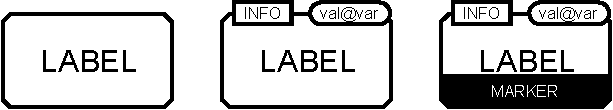
\includegraphics{images/complex-combined}
  \caption{The \PD glyph for \glyph{complex}, shown plain and unadorned on the left, with an additional \glyph{state variable} and a \glyph{unit of information} in the middle, and with a \glyph{labelled clone marker} on the right.}
  \label{fig:complex}
\end{figure}

% The following is for [X]Emacs users.  Please leave in place.
% Local Variables:
% TeX-master: "../sbgn_PD-level1"
% End:
